\section{Experimental evaluation}
\label{section:experiments}

In this section we will discuss the performance related issues of our 
HIPv2 implementation. We begin the discussion with the set of 
microbanchmarkings. Thus, we first evaluate the performance of ECDH and DH
algorithms, then we switch to performance of RSA, DSA, and ECDSA signature
algorithms, we conclude the discussion with the performance of various HMAC 
algorithms.

\begin{figure}
	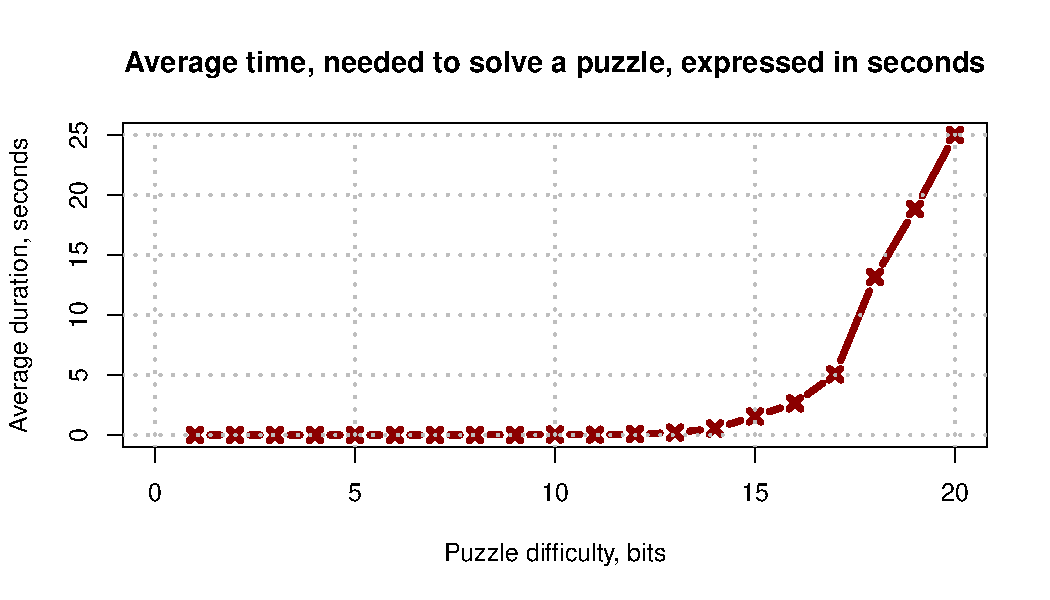
\includegraphics[width=0.5\textwidth]{graphics/puzzle_solution_perf.pdf}
	\caption{Average duration of puzzle solving}
	\label{fig:puzzle}
\end{figure}

To demonstrate the performance of ECHD and DH algorithms we have 
executed the key exchange algorithms $100$ times for various 
groups. Thus, in Figure~\ref{fig:dh} we show the performance of
DH and in Figure~\ref{fig:ecdh} we show the performance 
of ECDH for various curve parameters. To understand how two
are related in Table~\ref{tab:strength} we show the sizes
of various keys and how they are related to symmetric keys.
Obviously, ECDH shows far better performance than regular
DH algorithm. This performance improvement is largely due
to reduced key sizes.

\begin{figure}
	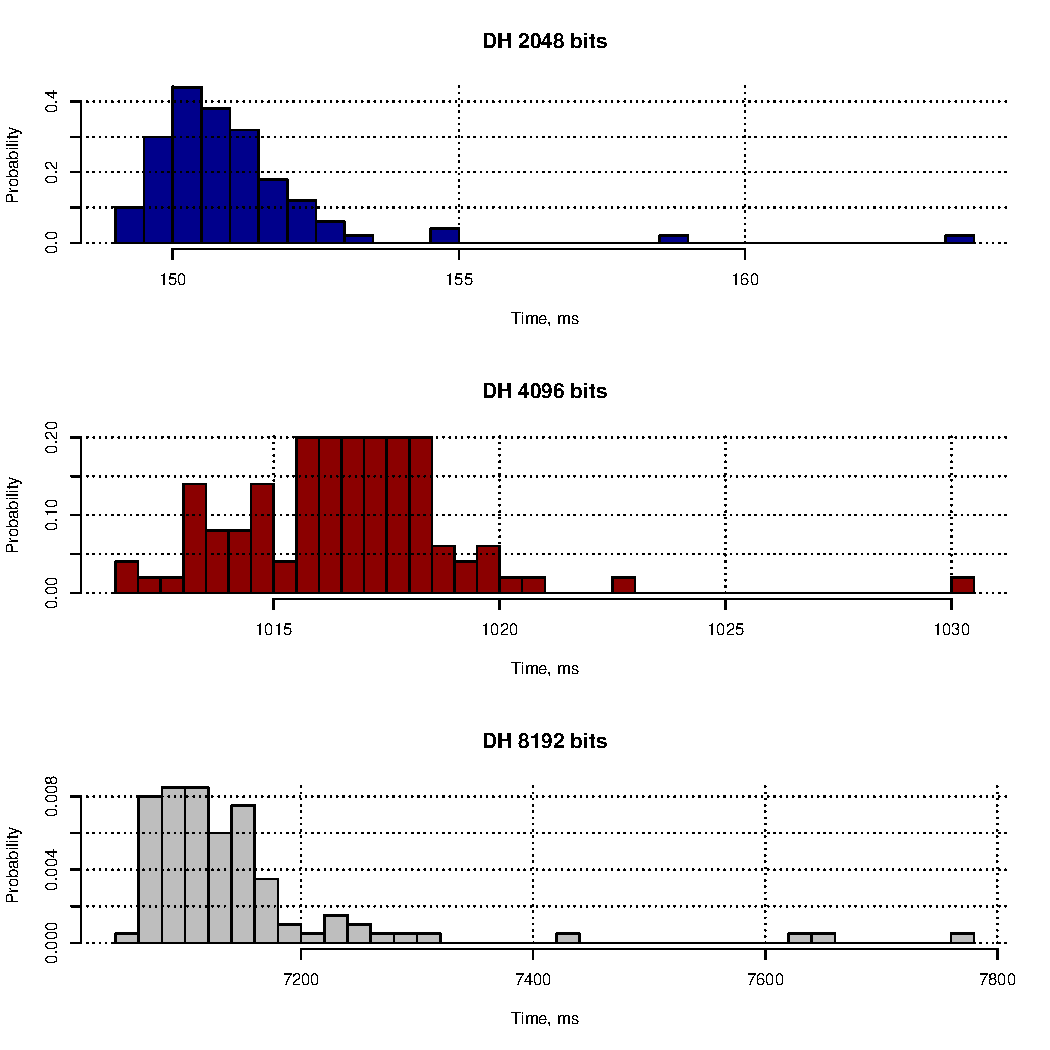
\includegraphics[width=0.5\textwidth]{graphics/dh_computation_hist.pdf}
	\caption{Diffie-Hellman key exchange duration (total)}
	\label{fig:dh}
\end{figure}

\begin{figure}
	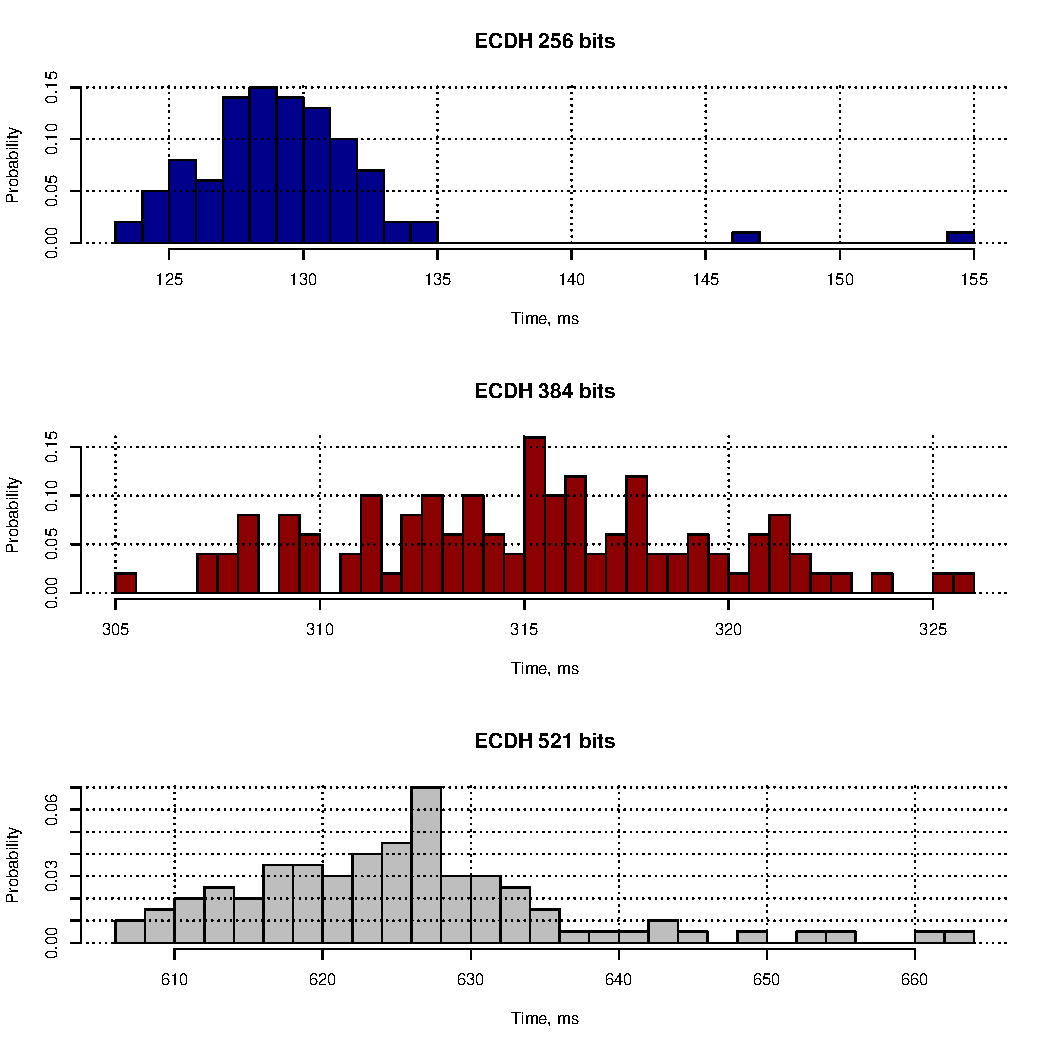
\includegraphics[width=0.5\textwidth]{graphics/ecdh_computation_hist.pdf}
	\caption{Elliptic Curve Diffie-Hellman key exchange duration (total)}
	\label{fig:ecdh}
\end{figure}

\begin{table}
\centering
\begin{tabular}{|c|c|c|}
\hline
\bf{Symmetric key sizes, bits} & \bf{DH keys, bits} & \bf{ECDH keys, bits} \\\hline
		80			&    1024                        & 160                                  \\
		112			&    2048                        & 224                                  \\
		128			&    3072                        & 256                                  \\
		192			&    7680                        & 384                                  \\
		256			&    15360                       & 521                                  \\
\hline
\end{tabular}
\caption{Security strength of keys}
\label{tab:strength}
\end{table}


\begin{figure}
	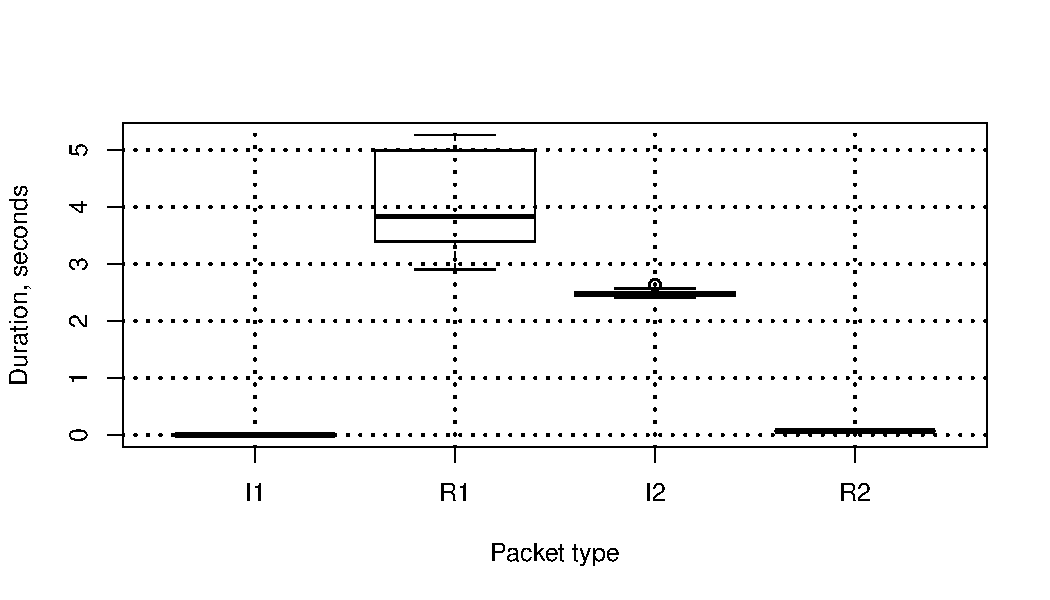
\includegraphics[width=0.5\textwidth]{graphics/packet_processing.pdf}
	\caption{Packets' processing time}
	\label{fig:packet_processing}
\end{figure}

We have ran the HIPv2 BEX for 20 times and measured the total packet processing time (we have combined packet 
processing time for initiator and responder). In Figure~\ref{fig:packet_processing} we show the boxplots for 
the packet processing duration. To run the tests we have used the following configuration: for signatures 
we have used RSA with $2048$ bits long modulus, SHA-256 for HMAC and hashing, ECDH with NIST521 curve, 
AES-256 for encryption and $16$ bits for puzzle difficulty. We have noticed that processing R1 packet consumes considerable
amount of time on responder. Since our implementation was lacking pre-creation of R1 packets, such lengthy packet 
processing time was expected. We have also measured the overall duration of the HIPv2 base exchange (BEX). 
In Figure~\ref{fig:duration_bex} we demonstrate distribution of HIP BEX durations. Clearly, implementing 
cryptographic protocols in userspace using high-level languages, such as Python, is not the best choice: the performance
of such implementations is really poor and it is better to implement the security solutions using lower 
level languages, such as C or C++.

\begin{figure}
	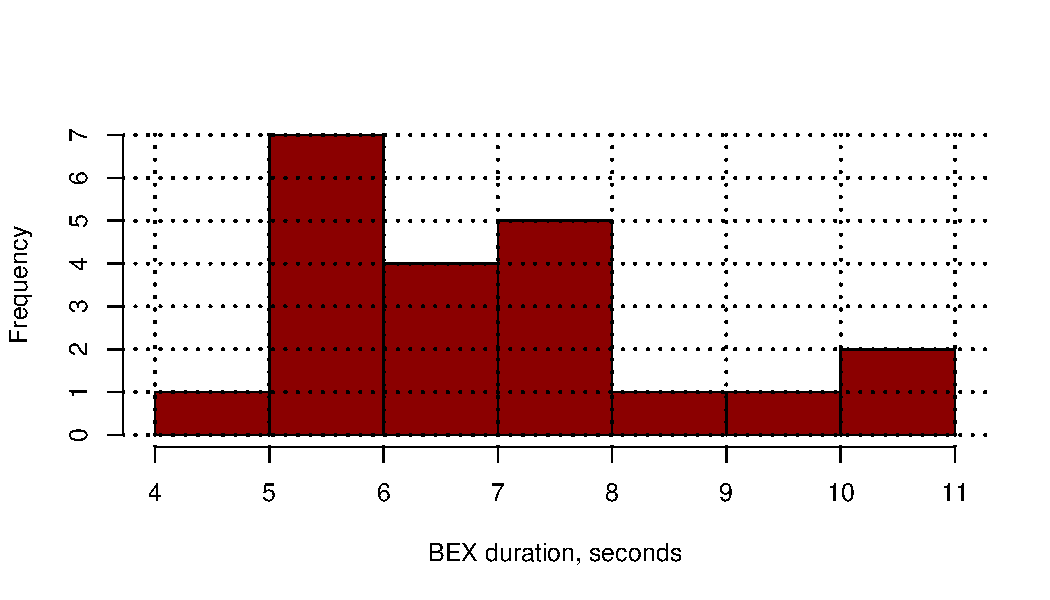
\includegraphics[width=0.5\textwidth]{graphics/duration_bex.pdf}
	\caption{Duration of HIPv2 BEX}
	\label{fig:duration_bex}
\end{figure}

Finally, we have measured throughput for TCP connections over IPSec tunnel and plain TCP. We have used
\texttt{iperf} tool to measure throughput. Clearly, our implementation of IPSec allows to achieve
throughput over $15$ times less, than throughput for plain TCP connections.

\begin{figure}
	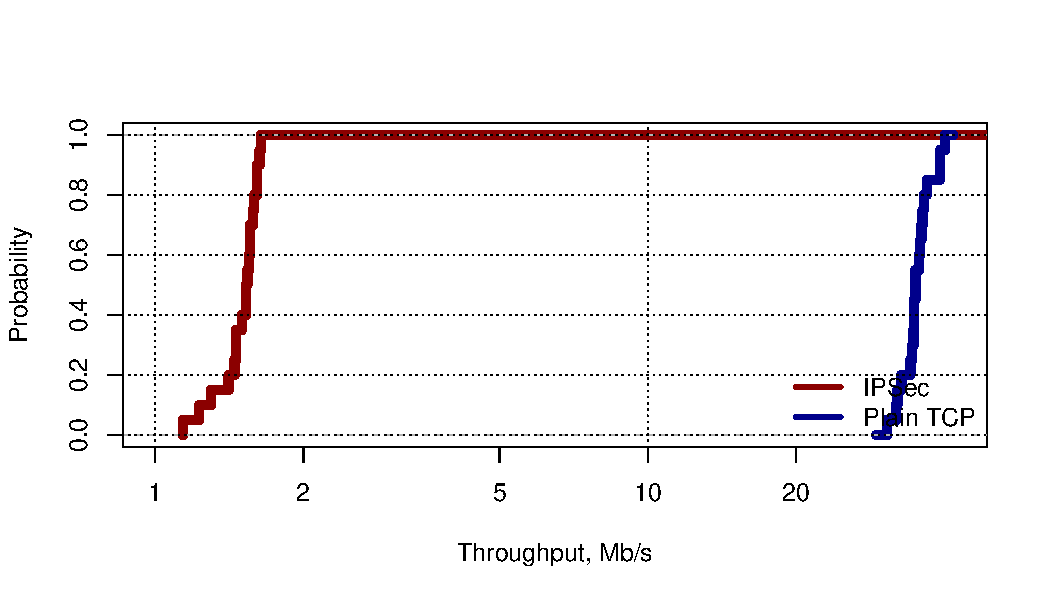
\includegraphics[width=0.5\textwidth]{graphics/throughput.pdf}
	\caption{Obtained throughput for TCP over IPSec and plain TCP connections}
	\label{fig:throughput}
\end{figure}
